\section{Bionische Oberflächen: Haftung und Antihaftung nach dem Vorbild der Natur}

\subsection{Superhydrophile Oberflächen}

\subsubsection{Am Beispiel der Wüstenechsen}

Wenn Wassertropfen die Oberfläche benetzen (sodass wir den Kontaktwinkel nicht mehr messen können), deutet das auf superhydrophile Oberflächen hin. Dies sehen wir z.B.\ bei den Schuppen von Wüstenechsen wie dem Dornenteufel (zweite Reihe im nächsten Bild links), der Texas-Krötenechse (dritte Reihe), etc. In der ersten Reihe ist zum Vergleich ein Wassertropfen auf den Schuppen einer nicht in der Wüste lebenden Eidechsenart dargestellt. Bei dieser Art hat sich die Funktion der hydrophilen Oberfläche nicht entwickelt.

\begin{center}
    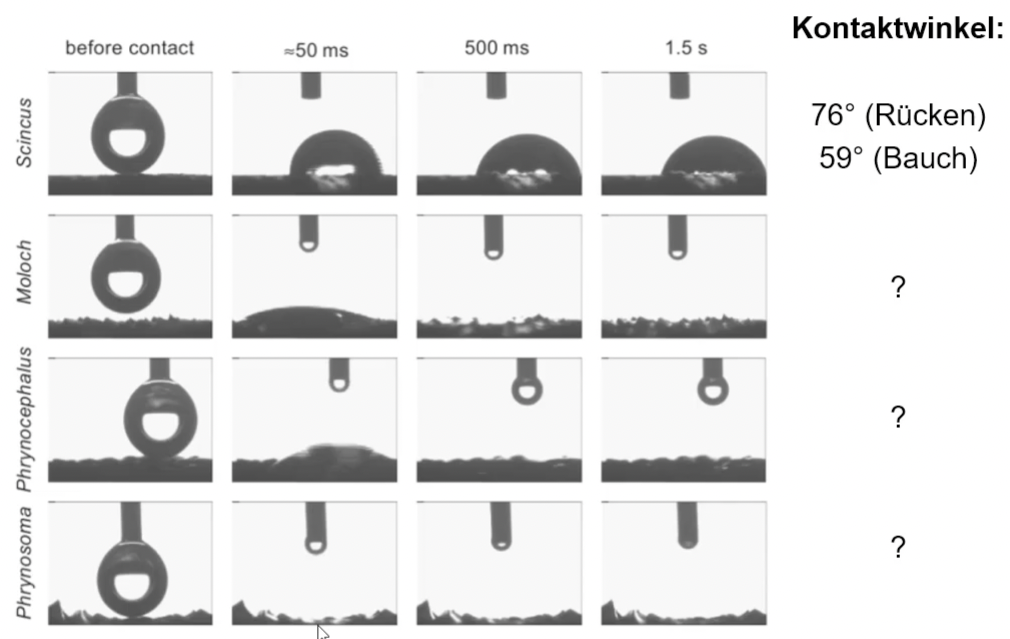
\includegraphics[width=10cm]{lec3/figures/Benetzung.png}
    \hfill
    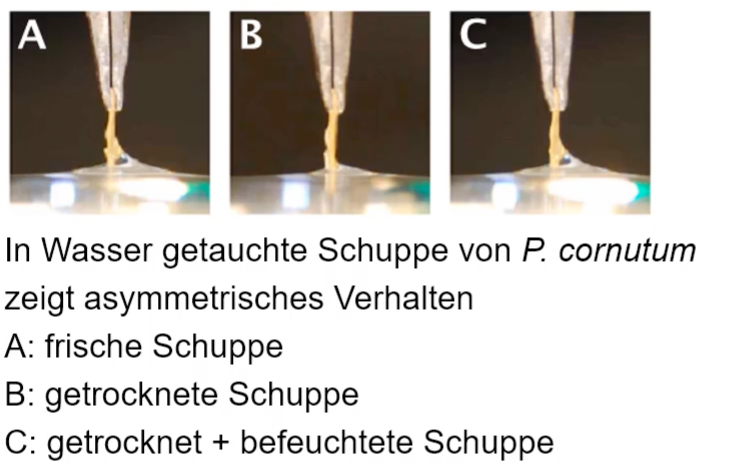
\includegraphics[width=6cm]{lec3/figures/Tauchen.png}
\end{center}
In dem rechten Bild ist ein Versuch zu sehen, bei dem 3 Schuppen in Wasser getaucht werden. Je nach Typ entstehen dabei unterschiedliche Kontaktwinkel, wobei der Innenbereich der Schuppe immer größere Kontaktwinkel als der Außenbereich hat. Da dieses Verhalten mit der unterschiedlichen Oberflächenstruktur zwischen Innen- und Außenbereich (Außenbereich zeigt Honigwaben-Mikrostruktur, Innenbereich nicht) korelliert, können wir hier die Ursache für den Effekt \textit{vermuten}.\\

Um diesen Zusammenhang nun zu beweisen, müssten wir genug kritische Versuche durchführen, welche die Vermutung nicht widerlegen. Ein möglicher Versuch, ist die Abformung der Mikrostrukturen mit Harz. Im nächsten Bild benetzt der Wassertropfen auf der abgeformten Funktionsoberfläche das Harz (oben), während der Tropfen auf der strukturlosen, ungeformten Rückseite des Harzes einfach abfließt (unten).

\begin{center}
    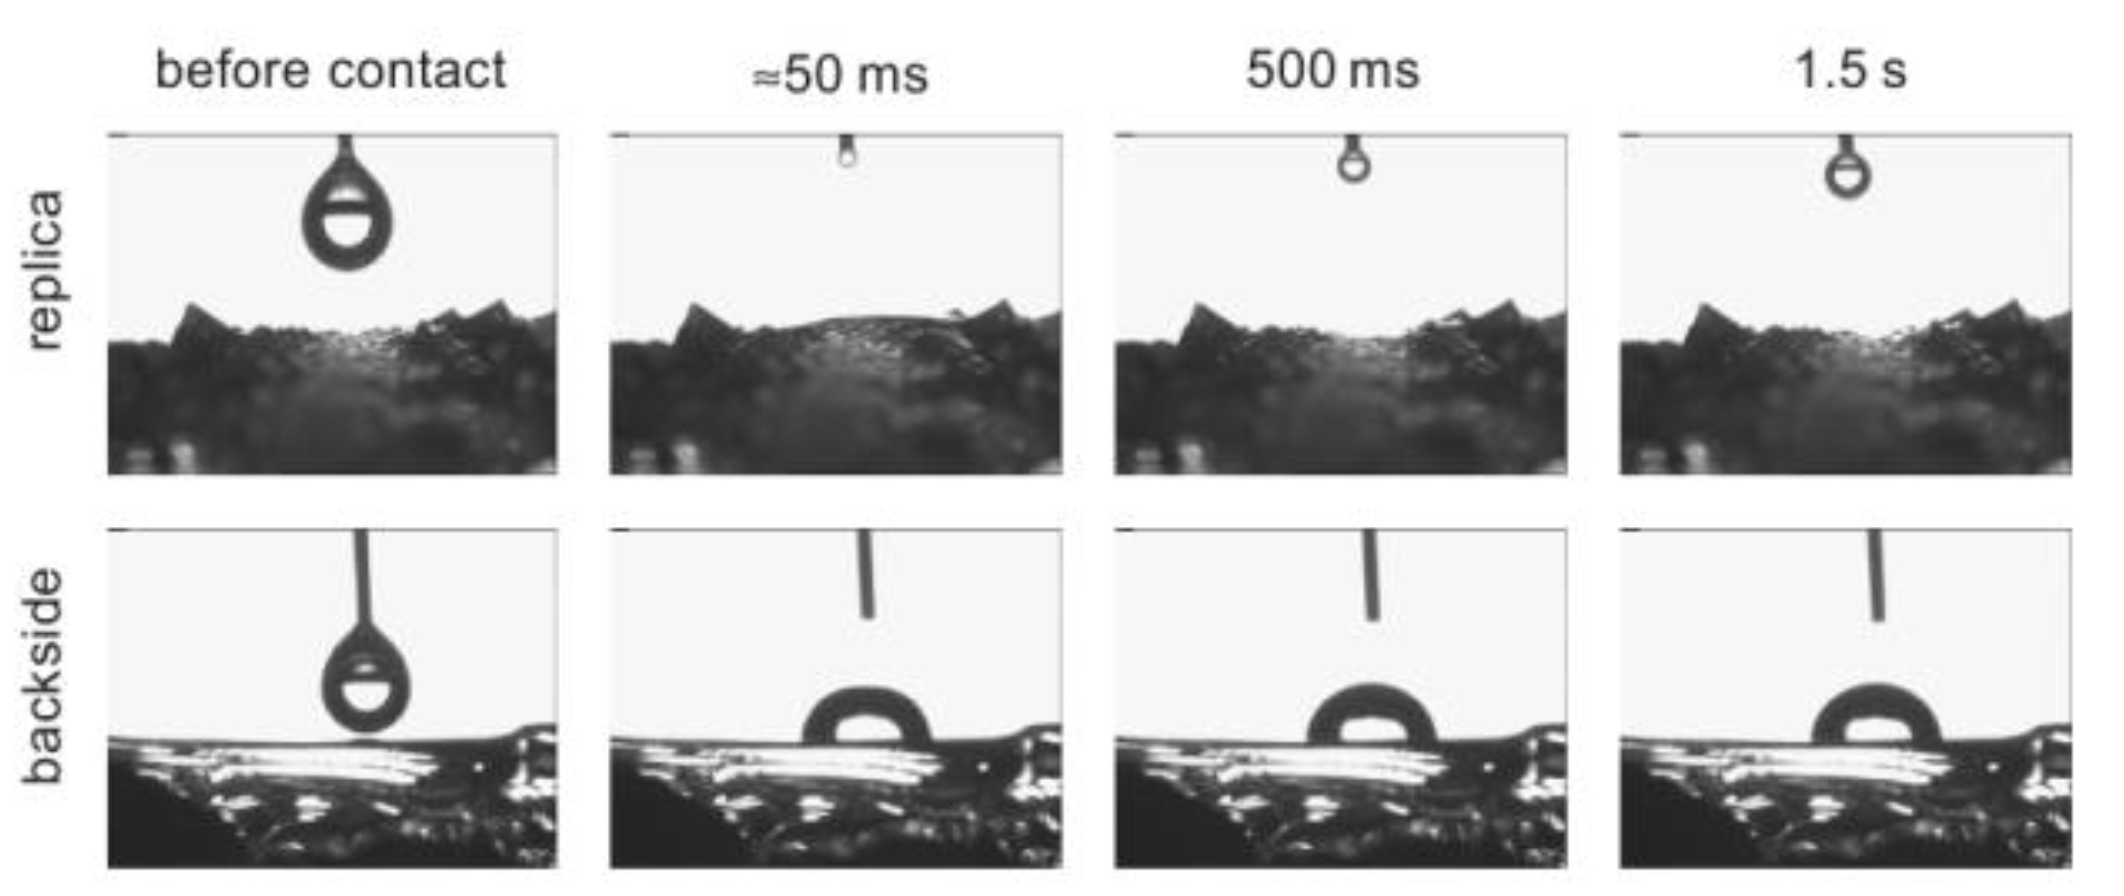
\includegraphics[width=10cm]{lec3/figures/Resin.png}
\end{center}

\paragraph{Wie kommt der richtungspezifische Transport von Flüssigkeit auf den Schuppen zustande?} Bei gewissen Arten wird Flüssigkeit Richtung Maul transportiert. Der Zwischenschuppen-Kanal (im linken Bild unten b; Spalt zwischen zwei Schuppen) weißt kleine Kerben (c) auf, deren Querschnit in Richtung des Mauls immer geringer wird. Es ergibt sich ein sägezahnförmiger Kanal (rechtes Bild). Die Flüssigkeit fließt aufgrund der Kapillarwirkung stets in Richtung der Verengung. (\dangersign \textit{Wie funktioniert der Richtungstransport von Wasser bei der Texas-Krötenechse?}) 

\begin{center}
    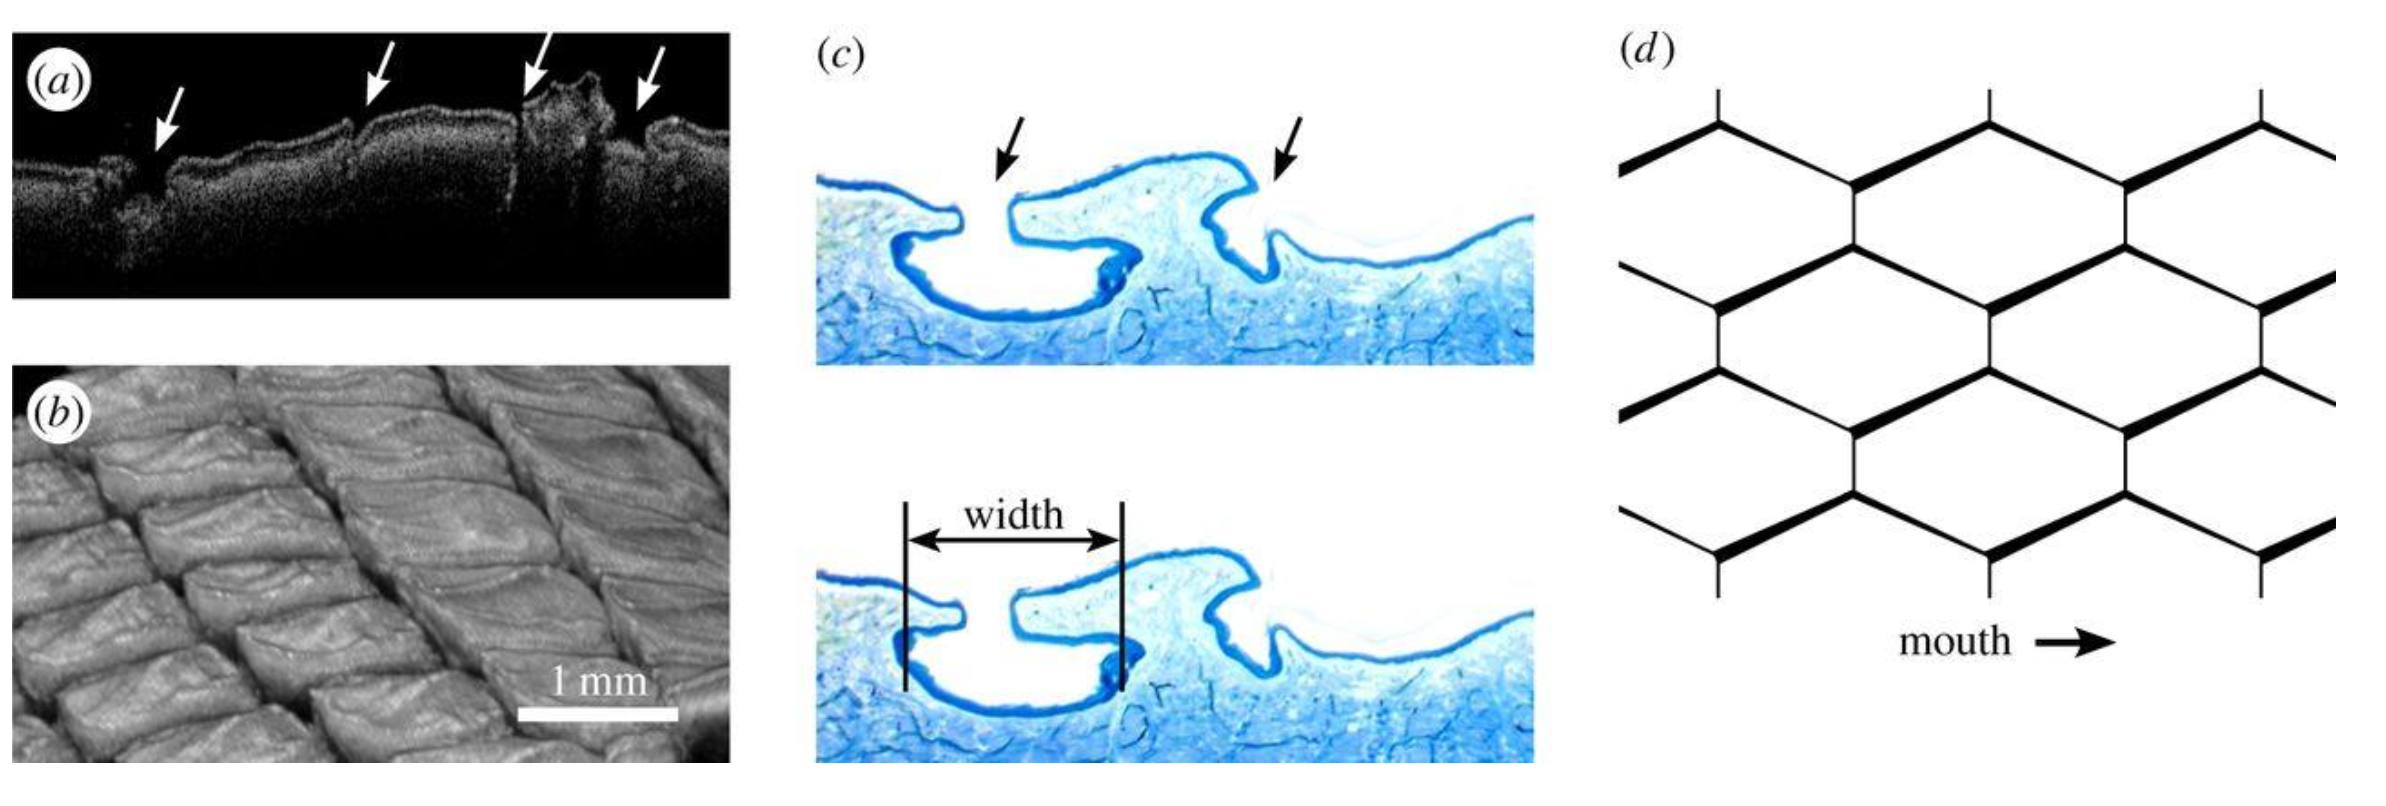
\includegraphics[width=10cm]{lec3/figures/Kerben.png}
    \hfill
    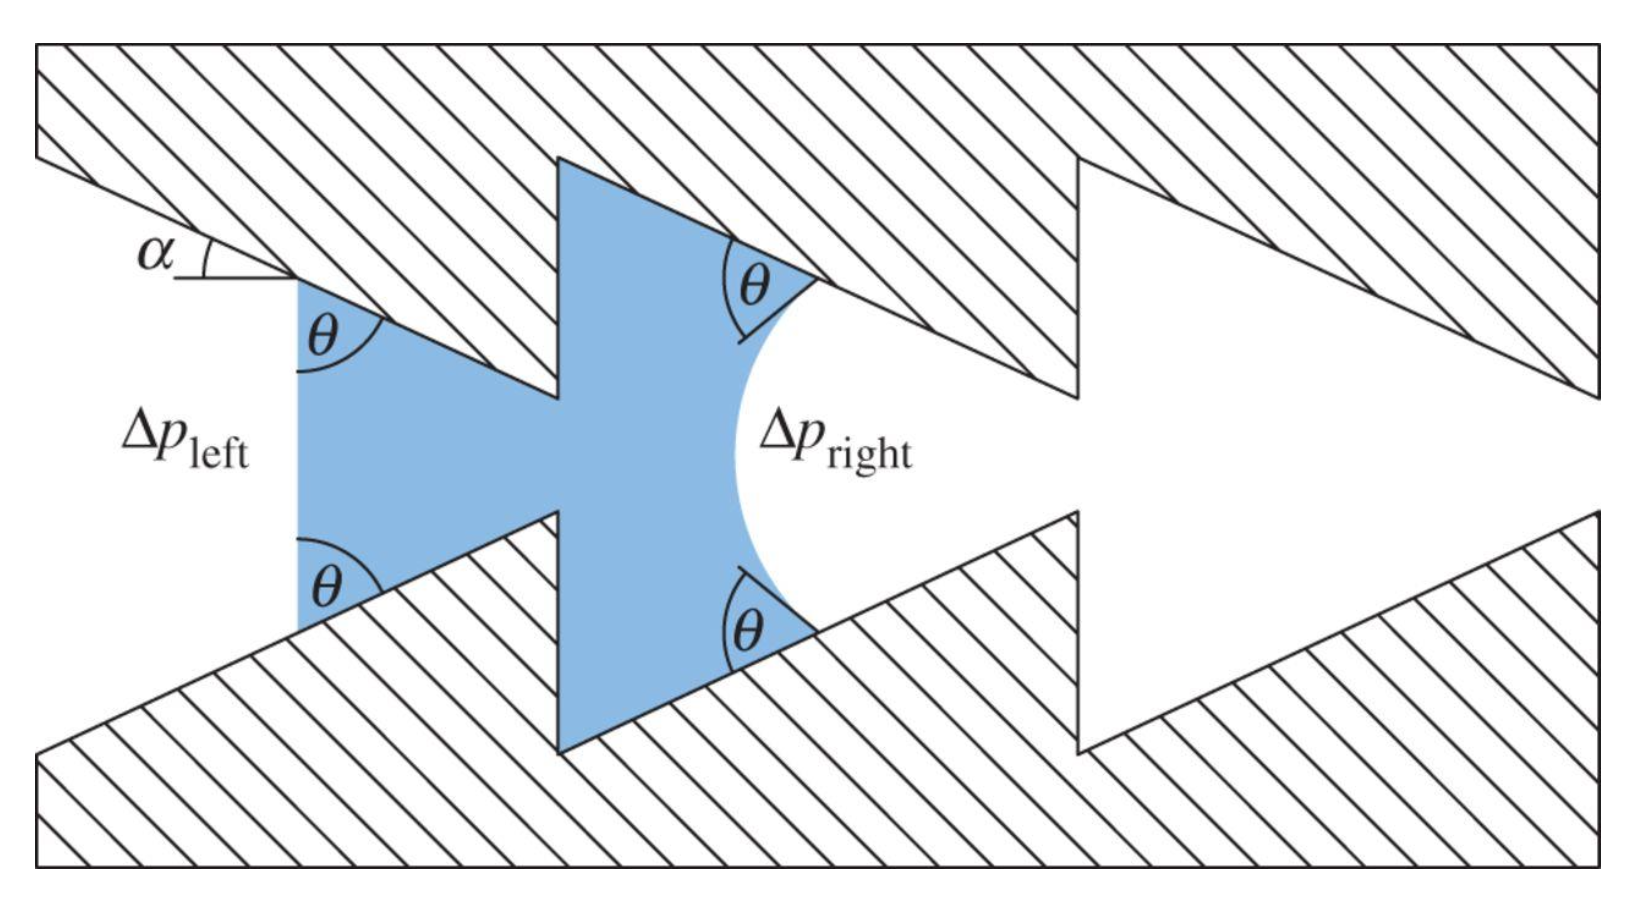
\includegraphics[width=6cm]{lec3/figures/Kanal.png}
\end{center}

\textit{Wie lässt sich das technisch nutzen} \dangersign? Sportbekleidung, die den Schweiß in Körperbereiche bringt, die gekühlt werden sollen. Oder zur verbesserten Verteilung von Flüssigkeiten auf Metall z.B.\ Öl, Kühlmittel (Einbringung per Laserstrahlstrukturierung, etc.) 

\subsubsection{Modelle zur Beschreibung des Benetzungsverhaltens}

Das \textbf{Wenzel-Modell} versucht den \textcolor{red}{Einfluss von Mikrostrukturierung auf das Benetzungsverhalten} zu erklären \dangersign, wobei die Flüssigkeit zwischen den Mikrostrukturen eindringt. Dabei errechnet sich der Kontaktwinkel der strukturierten Oberfläche $\theta_m$ nach:

$$\cos \theta_m = r \cos \theta,$$

wobei $\theta$ der Kontaktwinkel der glatten Oberfläche und $r$ der Quotient aus tatsächlicher Fläche (``von oben sichtbare Fläche'') und projizierter Fläche (ges. Oberfläche der Mikrostrukturen) ist. Die \textbf{Strukturierung führt bei chemisch hydrophilen Oberflächen dazu, dass die superhydrophil werden}. Allerdings kann das Modell bei den beschriebenen Echsenarten das Benetzungsverhalten nicht erklären. Wenn der Wassertropfen hängen bleibt ($\Longrightarrow$ Petal-Effekt, superhydrophobe Oberfläche die das Abrollen des Tropfen verhindert).\\

Bei dem \textbf{Cassie-Modell} sprechen wir von einer heterogenen Benetzung. Hier dringt die Flüssigkeit nicht zwischen die Mikrostrukturen ein ($\Longrightarrow$ Lotus Effekt, superhydrophobe Oberfläche).\\

Bei der \textbf{Cassie-Imprägnierung} dringt die \textcolor{red}{Flüssigkeit auch zischen die Mikrostrukturen ein, breitet sich darüber aus} \dangersign und macht die Oberfläche \textbf{superhydrophil}. Bei den Eidechsen kann mit dem Cassie-Impregnierungs-Modell das superhydrophile Benetzungsverhalten erklärt werden.

\begin{center}
    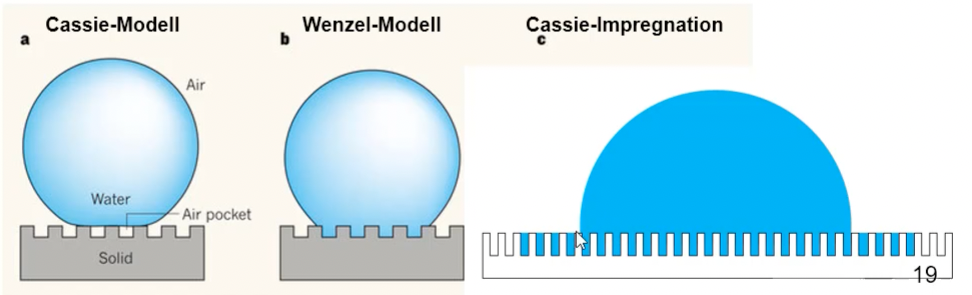
\includegraphics[width=10cm]{lec3/figures/wenzel_cassie.png}
\end{center}

\subsection{Lagebezeichnungen}
In der Biologie werden bestimmte \textbf{Lagebezeichnungen} verwendet, um die Lage von Körperteilen zu beschreiben:
\begin{itemize}
    \item Medial = Innen
    \item Lateral = Außen
    \item Dorsal = Rücken (Bspl. Dorsalschuppen)
    \item ventral = Bauch
    \item caudal = Schwanz
    \item cranial = Kopf
    \item proximal = Nah am Körper
    \item distal = Weit weg vom Körper
\end{itemize}

\subsection{Reversible Anhaftung nach dem Gecko- und Insektenfußprinzip}

\textbf{Adhesion} = trockenes Kleben (reversible Anhaftung).

Die Komplexität der Strukturierung nimmt hierarchisch von der Makro- zur Nanoebene zu \dangersign. Sowohl bei Geckos, als auch bei manchen Insekten findet sich diese hierarchische Gliederung und das Anhaften an unterschiedlichen Oberflächen. Feine Strukturen (\textcolor{red}{Lamella $\rightarrow$ Setae $\rightarrow$ Spatulae} im Bild unten) liegen eng an der Kontur der Oberfläche an, sodass sich van der Waals-Kräfte einstellen. Dieser schwache Anziehungseffekt stärkt die Adhesion.

\begin{center}
    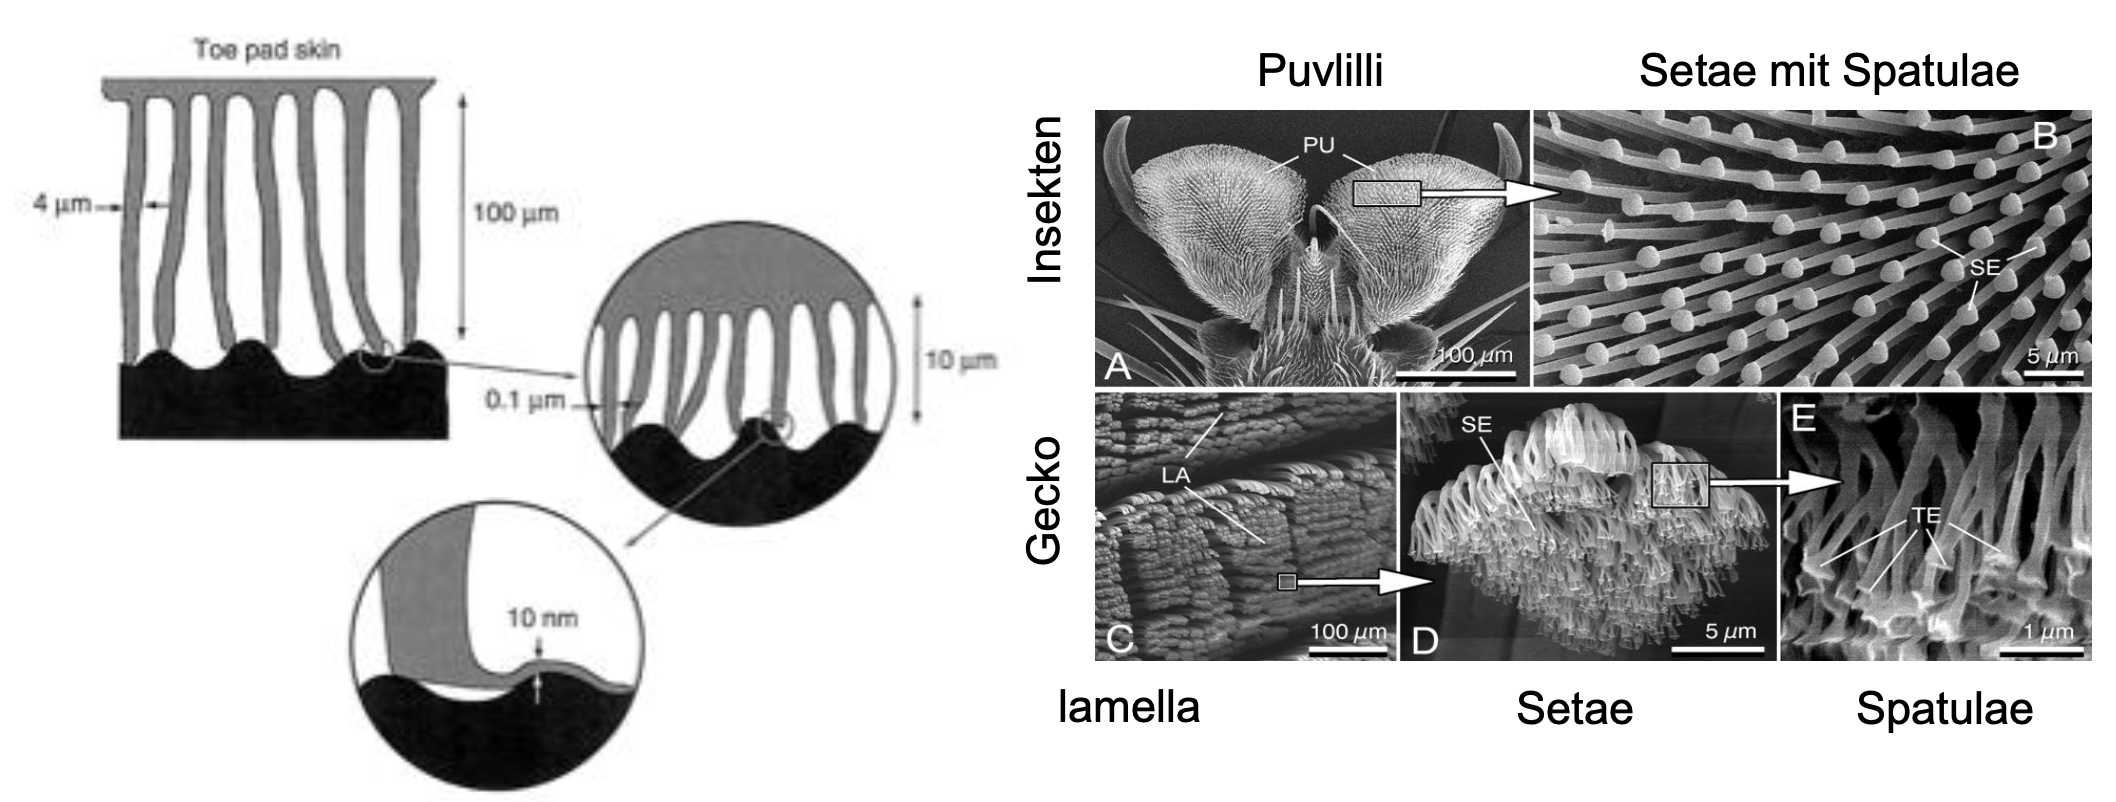
\includegraphics[width=10cm]{lec3/figures/vanderwaals.png}
    \hfill
    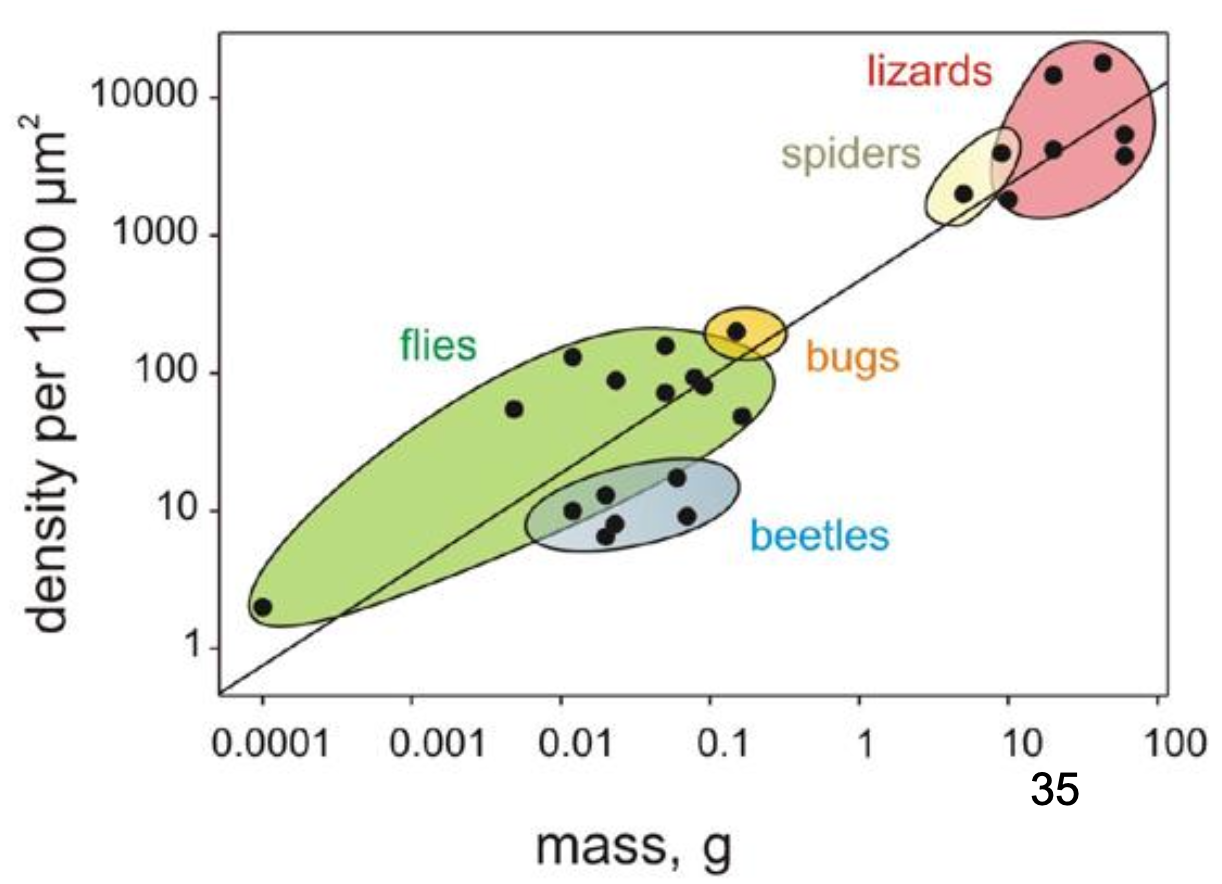
\includegraphics[width=6cm]{lec3/figures/setadichte.png}
\end{center}
Untersuchungen zeigen: Je schwerer das Tier ist, desto höher ist die Seta-Dichte, um das Gewicht des Tieres zu halten (siehe das Bild oben rechts). 
\\\\
\textit{Eine technische Anwendung}\dangersign: Das \textbf{``Gecko-Tape'' besitzt eine Oberfläche mit Setae-Strukturen}. Dabei stellte sich heraus, dass Setae mit \textbf{Pilzkopf-Form} (dem Kartoffelkäfer nachgearmt) besser haften.

\begin{center}
    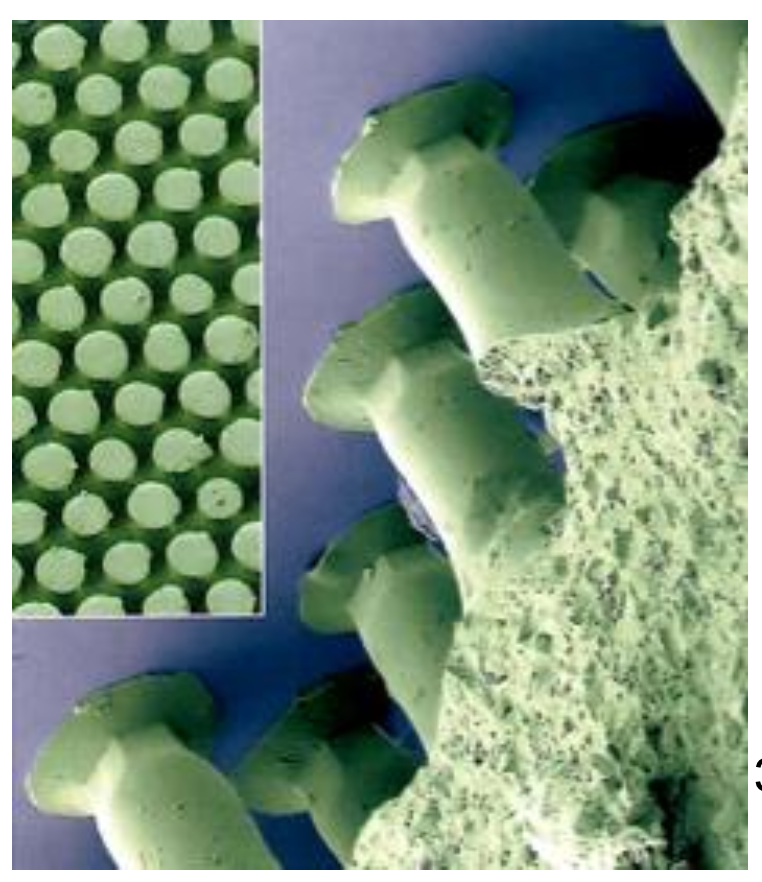
\includegraphics[width=3cm]{lec3/figures/pilzkopfform.png}
\end{center}





